\chapter{Interessante Recherche}
Während unser Recherche sind wir auf mehrere Studien \cite[S.129]{Benmimoun.2004} bezüglich der Kooperationsbereitschaft gestoßen. Das Saulendiagramm (Abb. \ref{fig:kooperation}) gibt die Druchsschnittsgeschwindigkeit in Abhängigkeit der Eingangsverkehrsstärke, sowie des Kooperationsanteils an. Auffallend ist, dass abhängig von der Verkehrsdichte unterschiedliche Kooperationsanteile einen besseren Verkehrsfluss bieten. Bei einer Eingangsverkehrsstärke von bis zu 15\,$\frac{\text{Fahrzeugen}}{\text{min}}/\text{Spur}$ hat der Kooperationanteil noch keinen großen Einfluss auf den Verkehrsfluss. Unabhängig von ihrem Fahrverhalten passieren die Fahrzeuge die Engstelle mit ca. 115\,$\frac{\text{km}}{\text{h}}$ bei einem Eingangsverkehr von 10\,$\frac{\text{Fahrzeugen}}{\text{min}}/\text{Spur}$ beziehungsweise ca. 105\,$\frac{\text{km}}{\text{h}}$ bei 15\,$\frac{\text{Fahrzeugen}}{\text{min}}/\text{Spur}$.
Bei 20\,$\frac{\text{Fahrzeugen}}{\text{min}}/\text{Spur}$ ist die Durchnittsgeschwindigkeit am besten, wenn sich genau 50\% der Autofahrer an das Reißverschlussverfahren nach StVO halten. Überraschend ist, dass der Verkehrsfluss besser ist, wenn sich nur 15\% der Verkehrsteilnehmer an die Vorschriften halten, als wenn sich 85\% dran halten. Dieses Phanomen ändert sich jedoch ab einer Eingangsverkehrsstärke von 25\,$\frac{\text{Fahrzeugen}}{\text{min}}/\text{Spur}$, bei welcher die bestmögliche Durchschnittsgeschwindigkeit von 50\,$\frac{\text{km}}{\text{h}}$ bei hoher Kooperaionsbereitschaft existiert.\\
\begin{figure}
	\centering
	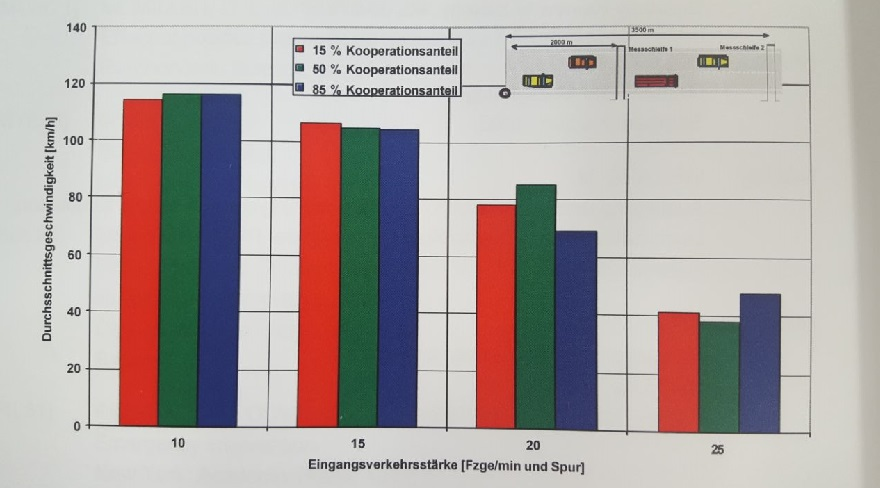
\includegraphics[width=0.6\linewidth]{images/Kooperation}
	\caption{Durchschnittsgeschwindigkeit im Szenario "'Autobahn bei hoher Dynamik und Dichte"'}
	\label{fig:kooperation}
\end{figure}
%FAT Schriften Reihe Nr. 181
%Effizienzsteigerung durch professionelles/ partnerschaftliches Verhalten im Straßenverkehr
%Auftragsgeber: Forscchungsvereinigung Automobiltechnik e.V. (FAT)
%Autor Ahmed Denmimoun, Dirk Neunzig, Christian Maag
%ISSN 0933-050 X
%2004
Diese Studie unterstreicht die Wichtigkeit, Fahrertypen zu implementieren, die einen unterschiedlichen Kooperationsanteil besitzen um ein realistisches Ergebnis zu erhalten.